% =============================================================================
% regression-scatter.tex — Scatter plot with OLS fit and confidence band
%
% Shows: bivariate scatter with fitted line and shaded confidence region.
% Uses \foreach to generate points; no real data.
%
% Compiles standalone via: xelatex regression-scatter.tex
% =============================================================================

\documentclass[border=4pt]{standalone}
\usepackage{tikz}
\usetikzlibrary{arrows.meta}

\definecolor{point}{HTML}{012169}
\definecolor{fit}{HTML}{B23A48}
\definecolor{band}{HTML}{F2C6CA}
\definecolor{axis}{HTML}{1A1A1A}

% -----------------------------------------------------------------------------
% Diagram: scatter over x ∈ [0, 8], y ∈ [0, 5].
% Fit: y = 0.5 + 0.55x. CI band: ±0.5 around the fit.
% Axes extend 0.3cm beyond data range (prevention rule P3 corollary).
% -----------------------------------------------------------------------------

\begin{document}
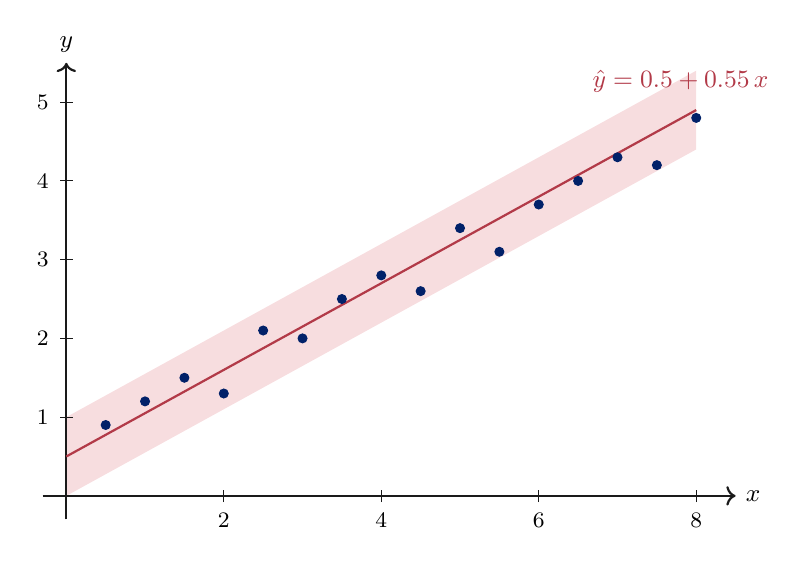
\begin{tikzpicture}
  % Confidence band (behind)
  \fill[band, opacity=0.6] (0, 0.5-0.5) -- (0, 0.5+0.5)
    -- (8, 4.9+0.5) -- (8, 4.9-0.5) -- cycle;

  % Axes
  \draw[->, thick, draw=axis] (-0.3, 0) -- (8.5, 0) node[right] {\small $x$};
  \draw[->, thick, draw=axis] (0, -0.3) -- (0, 5.5) node[above] {\small $y$};

  % Tick marks
  \foreach \x in {2, 4, 6, 8} {
    \draw[draw=axis] (\x, -0.08) -- (\x, 0.08);
    \node[below, font=\footnotesize] at (\x, -0.1) {\x};
  }
  \foreach \y in {1, 2, 3, 4, 5} {
    \draw[draw=axis] (-0.08, \y) -- (0.08, \y);
    \node[left, font=\footnotesize] at (-0.1, \y) {\y};
  }

  % Fit line: y = 0.5 + 0.55x  → endpoints (0, 0.5) and (8, 4.9)
  \draw[thick, draw=fit] (0, 0.5) -- (8, 4.9);

  % Scatter points (explicit coordinates so the snippet compiles deterministically)
  \foreach \x/\y in {
    0.5/0.9, 1.0/1.2, 1.5/1.5, 2.0/1.3, 2.5/2.1, 3.0/2.0,
    3.5/2.5, 4.0/2.8, 4.5/2.6, 5.0/3.4, 5.5/3.1, 6.0/3.7,
    6.5/4.0, 7.0/4.3, 7.5/4.2, 8.0/4.8
  } {
    \filldraw[point] (\x, \y) circle (1.6pt);
  }

  % Fit label — placed above-right of the line at x = 7.5 to avoid scatter.
  \node[above, fit, font=\small] at (7.8, 5.0) {$\hat{y} = 0.5 + 0.55\,x$};
\end{tikzpicture}
\end{document}
